\documentclass{practicaitic}
\usepackage{parskip}
\usepackage{graphicx}

\usepackage[onelevel]{exercici}
%\usepackage[utf8]{inputenc}

\usepackage{tcolorbox}

\numpract{3}
\title{Pràctica 4: Servei de correu}

\assignatura{Aplicacions i Serveis sobre Internet}
\autor{Eric Roy Almonacid \and Francisco del Águila López}

\begin{document}

\section{Introducció}

Per poder realitzar aquesta pràctica és indispensable haver completat la
pràctica 1 i 3, donat que treballarem sobre el VPS i domini creats anteriorment.

\begin{tcolorbox}[
  title=Atenció,
  colback=red!10, colframe=red!50,
  rounded corners
]
Per aquesta pràctica el servidor hauria de poder enviar paquets TCP al 
ports del servei de correu, d'entre els quals el port 25. Si utilitzeu
\textit{Hetzner}, haureu de realitzar una petició
per desbloquejar els ports a la secció de \textit{Limits}.
La \href{https://docs.hetzner.com/robot/dedicated-server/faq/faq#why-can-i-not-send-any-mails-from-my-server}{documentació de \textit{Hetzner}} demana que els usuaris tinguin una
antiguitat superior a un mes per treure els límits.
\newline

Si no aconseguiu desbloquejar l'accés a aquests ports dirigiu-vos a
l'apartat \ref{sec:plan-b}.
\end{tcolorbox}

\subsection{Objectius}

Al finalitzar aquesta pràctica, l'estudiantat haurà:
\begin{enumerate}
  \item Entès el funcionament i l'arquitectura del servei de correu.
  \item Utilitzat \texttt{exim} o \texttt{postfix} per enviar correus de forma local.
  \item Configurat un servidor de recepció de correus obert a Internet.
  \item Configurat l'enviament de correus a Internet des del servidor sense
  utilitzar \textit{smarthosts} de tercers.
  \item Entès totes les tasques addicionals que cal dur a terme per
  esdevenir un remitent de correu fiable.
\end{enumerate}

\subsection{Condicions}

Aqeusta pràctica està cal·librada per ésser treballada en equips de 2 persones,
i té una durada de 2 setmanes.

\subsection{Lliuraments}

S'haurà de realitzar una entrega a Atenea i mantenir operatiu el servidor 
i domini creats fins que la pràctica sigui avaluada. El format de l'entrega
està detallat a l'apartat \ref{sec:entrega}.

\section{El correu electrònic}

El correu electrònic que coneixem avui es segueix basant en la
implementació original que va aparéixer a ARPANET l'any
1981, quan es va publicar les especificacions del protocol SMTP
(\textit{Simple Mail Transfer Protocol}). Aleshores, Internet consistia
en una xarxa amb molt pocs nodes i de difícil accés.

L'extensió d'Internet i la facilitat d'enviar correus massivament o bé
impersonant algú altre han obligat crear extensions de seguretat per
SMTP: des d'utilitzar TLS fins a autenticar els missatges en funció
de registres en el DNS. Hi ha molts factors a tenir presents si
es vol enviar correus electrònics a grans proveïdors com Gmail.
Tot plegat fa que ens puguem preguntar si la S de SMTP segueix
significant \textit{Simple}. % Paco: si vols pots treure aquesta frase :)

Aquesta pràctica pretén oferir una guia per poder convertir el vostre
VPS en un servidor de correu i així no haver de pagar mensualitats 
massa elevades per només disposar d'una adreça electrònica corporativa.
Hi ha projectes com \href{https://docs.mailway.app/self-host/}{MailWay} o 
\href{https://docs.mailcow.email}{MailCow} que permeten configurar un
servidor de correu en pocs passos, però en aquesta pràctica utilitzarem
\texttt{exim} o \texttt{portfix} per entendre realment què estem fent.

\subsection{La visió original}

Al ser un protocol que porta més de 40 anys en funcionament, és d'esperar
que SMTP tingui peculiaritats degudes als sistemes d'aquella època. Per
entendre el perquè d'algunes funcionalitats que veurem més endavant és
convenient dedicar uns paràgrafs al passat d'aquest sistema.

En el moment de la seva creació, la gran majoria d'usuaris només disposaven
d'un únic ordinador, sovint compartit amb altres persones, i només accedia
al correu a través d'aquest. Per tant, era lògic pensar que es podria
utilitzar la notació \texttt{usuari@maquina} com a identificador
per enviar correus. Si es vol una altra bústia, només cal crear un
nou usuari al sistema.

A més a més, cada ordinador tenia una adreça IP pública. Només calia
fer coincidir el \textit{hostname} de la màquina amb el nom de domini
d'aquesta i ja es disposaria d'un identificador accesible des de tot
arreu. Per això veurem que \texttt{exim} posa complicacions si volem
gesionar diversos noms de domini des d'un mateix servidor.

Finalment, cal tenir present que no tots els ordinadors estaven
encesos i encara menys connectats a internet tota l'estona (sobretot
quan les companyies de telefonia facturaven per temps d'utilització).
Així doncs, és possible que un usuari envii un correu electrònic a
una màquina que està apagada, i que estigui desconnectat quan l'altre
el pugui rebre. Per aquest motiu es van dissenyar els servidors MTA
(\textit{Mail Transfer Agent}) o \textit{smarthosts}, que rebien el
correu dels usuaris o MUA (\textit{Mail User Agent}) i s'encarregaven
de dur-lo al destinatari i esperar si feia falta.

Actualment, tot i seguir podent utilitzar servidors MTA com si res,
gairebé tots els servidors de correu estan sempre disponibles, pel
que han perdut la seva utilitat.

\subsection{Enviament en local}

El correu més bàsic que es pot enviar és entre dos usuaris de la
mateixa màquina. En aquest apartat configurarem el servidor
per poder enviar-vos correus entre els diferents integrants
del grup. En la major part d'aquesta pràctica utilitzarem \texttt{exim},
però podeu utilitzar qualsevol aplicació que compleixi el protocol.

\begin{previ}
  Insta\lgem eu-vos el paquets necessaris a la vostra màquina virtual:
  \texttt{exim4 default-mta}. Aquest darrer és un paquet virtual que
  conté \texttt{exim4-daemon-light} (MTA Exim) i \texttt{heirloom-mailx}
  (MUA mail).
\end{previ}

Sempre que vulguem consultar la configuració d'\texttt{exim4} utilitzarem la
comanda \texttt{debconf-show exim4-config}, i sempre que vulguem modificar-la
ho podrem fer a través d'una interfície mitjançant la comanda
\texttt{dpkg-reconfigure exim4-config}. Per a entendre les opcions,
consulteu \texttt{man update-exim4.conf} i la documentació a
\texttt{/usr/share/doc/exim4/README.Debian.gz}.

\begin{tasca}
  Executeu la comanda per configurar \texttt{exim4} i seguiu els passos
  per poder enviar i rebre correus entre els diferents usuaris de la
  mateixa màquina. A quines adreces IP s'haurà d'acceptar connexions SMTP?

  Redirigiu els correus de \texttt{root} als vostres usuaris mitjançant
  l'interfície anterior i comproveu que els canvis s'han aplicat llegint el
  fitxer \texttt{/etc/aliases}. Afegiu un nou àlies \texttt{tothom} que
  permeti enviar correus a tots els usuaris (alumnes i \texttt{profe})
  simultàniament.

  Utilitzeu la comanda \texttt{mail tothom} per enviar un correu electrònic a
  \texttt{tothom}, i comproveu que l'heu rebut amb \texttt{mail}. Fixeu-vos
  com canvien alguns valors de la capçalera del correu al utilitzar un àlies.
\end{tasca}

\begin{tcolorbox}[
  title=Atenció,
  colback=red!10, colframe=red!50,
  rounded corners
]
Al tenir una màquina connectada a internet, aquesta és vulnerable a atacs
externs. Si no es configura \texttt{exit} adequadament, aquest és capaç
d'acceptar correus provinents de desconeguts. Un dels possibles escenaris
és el que es mostra a la figura \ref{fig:escenari-malicios}, on el servidor
permet reenviar correus amb qualsevol domini i qualsevol usuari d'origen.
\newline

Us recomanem utilitzar el tallafocs per denegar tots els paquets de SMTP
entrants fins que estigueu convençuts que el servidor està ben configuat.
\end{tcolorbox}

\begin{figure}[h]
  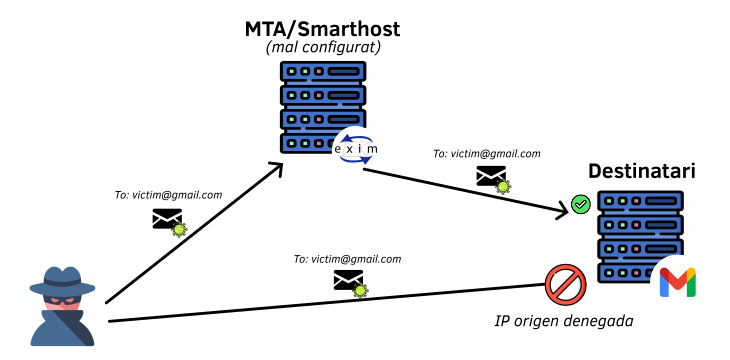
\includegraphics[width=0.6\linewidth]{assets/p4-escenari-malicios.png}
  \centering
  \caption{
    Una persona amb males intencions pot utilitzar un servidor de correu
    mal configurat per difondre massivament correus electrònics. A part de
    ser còmplices (indirectament) d'un atac, aconseguirem que la nostra adreça
    IP aparegui en llistes negres i tots els correus sortints estiguin rebutjats
    o vagin a parar al correu brossa.
    }
  \label{fig:escenari-malicios}
\end{figure}

\subsection{Recepció des d'Internet}

El següent pas serà poder rebre correus electrònics d'Internet. Evidentment,
només acceptarem correus que vagin destinats al nostre domini.

\begin{previ}
  Torneu a executar la comanda per configurar \texttt{exim4} per ara poder
  rebre correus de qualsevol adreça IP. Ara haureu d'usar el mode
  \textit{internethost}.

  Després, afegiu un registre MX que indiqui que els correus del domini
  del servidor s'han d'enviar al domini del servidor. Al només tenir un
  servidor que gestioni els correus d'aquest domini, no importa el valor
  de prioritat que indiqueu.

  Fixeu-vos que el registre MX es podria considerar com a redundant en aquests
  casos, donat que és idèntic que el registre A/AAAA. De totes formes, es
  recomana posar-lo igualment per augmentar la reputació del domini
  (vegeu apartat \ref{sec:reputation}), i perquè alguns servidors de
  correu només miren el registre MX.
\end{previ}

Recordeu modificar el tallafocs per permetre peticions entrants als ports
del protocol SMTP.

\begin{tasca}
  Envieu un correu des del vostre compte de la UPC (és a dir, Gmail) a
  l'àlies \texttt{tothom}. Fixeu-vos que Google, com la majoria de
  MUA, afegeix diversos camps addicionals al correu electrònic. Alguns
  seran de vital importància més endavant.

  Proveu d'enviar un correu a una adreça existent. Què succeeix? I si
  atureu el servidor i envieu un correu?
\end{tasca}

% \subsection{Us d'alies} % Finalment ho he integrat en els passos anteriors

% \begin{tasca}
%   Posar esutdiantat@ que redirigeixi als dos estudiants, tots@ també a profe. Enviar mail.
% \end{tasca}

\subsection{Enviament a través d'Internet}

Per poder completar el cicle només falta aconseguir enviar correus a l'exterior.
Si heu realitzat correctament la recepció de correus electrònics, ja haurieu
de poder enviar-ne.

\begin{previ}
  Comproveu que pugueu realitzar connexions sortints als ports de SMTP
  mitjançant \textit{netcat}. Potser haureu de demanar al proveïdor que
  us habiliti aquests ports.

  % nc -vv smtp.google.com 25
  % nc -vv smtp.google.com 465
\end{previ}

\begin{tasca}
  Envieu correus electrònics als servidors dels altres grups.
  Podeu inclús parlar-vos amb grups
  que no tinguin adreça pública, sempre i quan estigueu connectats
  a la VPN i tinguin associat un nom de domini a l'adreça IP pertinent.
\end{tasca}

\begin{tasca}
  Envieu un correu des del servidor a la vostra adreça personal de la UPC.
  Veureu que el rebreu a la carpeta de correu brossa.
  
  Si no el rebeu, segurament
  hagueu rebut una resposta per part de Gmail a l'adreça remitent (és a dir,
  al servidor) indicant quin és el probema (per exemple, que l'adreça IP està
  banejada). % Com es diu banned en català?
\end{tasca}

\subsubsection{Alternativa per si no es pot utilitzar els ports de SMTP}
\label{sec:plan-b}

Degut a l'abús que fan els criminals dels VPS per enviar correus
fraudulents, els proveïdors solen filtrar les connexions sortints
als ports de SMTP. Moltes vegades és suficient amb un missatge per
eliminar aquest límit, però en alguns casos aquests no s'aconsegueix.

Si vulguéssiu utilitzar el correu de forma comercial no tindríeu cap
altre remei que esperar o canviar de proveïdor, però els terminis
d'aquesta pràctica obliguen a trobar formes alternatives d'experimentar
amb SMTP.

Així doncs, pel que queda d'enunciat de la pràctica, si no podeu
enviar correus a través d'Internet amb els ports de SMTP, haureu de realitzar
totes les parts que pugueu entre diversos servidors disponibles a la mateixa
VPN: fixeu-vos que no podeu realitzar connexions al port 25 a Google, però sí
al rang de la VPN de l'escola.

\section{Servidor de correu amb bona reputació}
\label{sec:reputation}

Tal i com s'ha comentat en apartats anteriors, amb el pas del temps s'han
afegit diverses extensions al protocol SMTP per verificar que el correu en
qüestió és legítim. Alguns son protocols nous, altres son simplement bones
pràctiques.

En l'actualitat és escencial poder complir amb tots els requeriments que els
grans proveïdors de correu electrònic comproven per tal de tenir un servidor
de correu útil.

En aquest apartat es detalla tot el que s'ha de tenir present per deixar
d'apareixer a la carpeta de correu brossa.

\subsection{DNS invers}

\begin{tasca}
  Verifiqueu que el DNS invers de la IP del vostre servidor porta al domini
  del servidor (aquesta tasca ja la vau fer a la pràctica 3).
\end{tasca}

\subsection{Blacklists}

La majoria de servidors de correu rebutgen correus si aquests apareixen a
llistes negres d'adreces IP. Hi ha diverses llistes públiques que la majoria
de servidors de correu consulten.
A més a més, alguns proveïdors, com Google, fan servir llistes pròpies a part
de les mencionades anteriorment.

\begin{tasca}
  Utilitzeu una eina online (per exemple \url{https://mxtoolbox.com/blacklists.aspx})
  per comprovar si les adreces IPv4 i IPv6 del vostre servidor apareixen en una
  llista negra.
\end{tasca}

És molt probable (donat que no estem utilitzant una IP $100\%$ nova) que
estiguem en alguna llista. Caldrà doncs, llista per llista, sol·licitar
que es suprimeixi l'adreça del nostre servidor. No cal que us desapunteu
dels llocs on us demani pagar (si més no, no per aquesta pràctica).

La llista en la que apareixereu amb més probabilitat és la \textit{RATS-NoPtr},
una llista que apunta totes les adreces sense DNS invers configurat
correctament. Només cal configurar el DNS invers i omplir el formulari per
(al cap d'uns dies) desaparéixer d'aquesta llista.

\subsection{Verificació del remitent amb SPF}

SPF o \textit{Sender Policy Framework} és sens dubte l'extensió que més es miren
els proveïdors per determinar si un correu és legítim o no, degut a la seva
simplicitat. Consisteix en introduir un registre TXT al servidor de noms
que contingui la informació necessària per tal que un servidor de correu pugui
determinar si el correu rebut prové d'un remitent legítim o no.

Podem consultar utilitzant \texttt{dig} registres SPF d'altres dominis
(s'ha mostrat només els registres TXT útils per aquesta pràctica):

\begin{verbatim}
dig +short txt epsem.upc.edu
"v=spf1 mx ip4:147.83.2.50 ip4:147.83.2.51 ip4:147.83.2.77 ?all"
\end{verbatim}

Basant-se en la comanda anterior, els correus electrònics de la EPSEM
(a data d'abril de 2025) es poden enviar des de 3 adreces IPv4 diferents i
des de l'adreça (o adreces) que es puguin obtenir a partir del
registre MX del mateix domini.

La darrera paraula del registre sempre serà \texttt{all} i vindrà precedida per
un caràcter que determinarà el comportament de SPF:
\begin{itemize}
  \item \texttt{+all}: permet tot el trànsit (poc recomanat, indica \textit{pass}").
  \item \texttt{-all}: rebutja tot el trànsit no autoritzat explícitament (\textit{fail}).
  \item \verb|~all|: marca com a sospitós (posa en quarantena) el trànsit no autoritzat (\textit{softfail}).
  \item \texttt{?all}: no especifica cap política clara pel trànsit no autoritzat (\textit{neutral}).
\end{itemize}

Tambe es pot utilitzar \texttt{include} per incloure tots els remitents d'un altre
domini:

\begin{verbatim}
dig +short txt google.com
"v=spf1 include:_spf.google.com ~all"
\end{verbatim}

Podeu consultar el llistat detallat d'opcions pel registre SPF a
\url{https://support.google.com/a/answer/10683907} o al
\href{https://datatracker.ietf.org/doc/html/rfc7208}{RFC 7208}.

\begin{tasca}
  Configureu SPF al vostre domini per tal que s'acceptin correus sortint només
  del vostre servidor (IPv4 i IPv6). La resta de correus es poden deixar en
  quarantena.

  Proveu d'enviar de nou un correu electrònic a la vostra adreça de la UPC
  i comproveu si es segueix rebent al correu brossa o no (espereu-vos unes hores
  per assegurar-vos que s'hagin propagat els canvis del DNS).
\end{tasca}

\subsection{Signatura de correus amb DKIM}

Encara que amb la tasca anterior ja us apareguin els correus a la safata
d'entrada, per assegurar que això segueixi sent així cal realitzar dos passos
més.

DKIM o \textit{DomainKeys Identified Mail} és un sistema que permet signar
correus electrònics sortints per demostrar al destinatari que aquests no han
estat modificats.
Consisteix en deixar una clau pública en un registre TXT del domini i signar
tots els missatges sortints amb la seva clau privada, emmagatzemada al servidor.

\begin{tasca}
  Configureu el vostre servidor de correu per utilitzar DKIM. Heu de:
  \begin{enumerate}
    \item Generar un parell de claus públiques i privades.
    \item Notificar a exim que utilitzi DKIM i indicar el lloc de la clau privada.
    \item Aplicar la configuració i reiniciar exim.
    \item Publicar la clau pública en un registre DNS.
  \end{enumerate}
\end{tasca}

Podeu seguir algun tutorial com el següent: \url{https://bobcares.com/blog/configuring-dkim-for-exim/}. Possiblement pel vostre cas hi haurà certs detalls
a canviar. Us pot ser útil consultar els errors i \textit{logs} que exim es
va trobant al fitxer \texttt{/var/log/exim4/mainlog}.

Pel darrer pas (publicar la clau pública al DNS), heu de copiar els continguts
del fitxer de la clau pública que hagueu generat al registrador de DNS en
forma de registre TXT a \texttt{<DKIM\_SELECTOR>.\_domainkey.<SERVIDOR>}, on 
haureu de reemplaçar el primer valor pel selector que hagueu utilitzat en el
fitxer de configuració d'Exim.

El resultat hauria de ser similar al següent. Compte! Elimineu tots els salts
del línia en el moment d'enganxar la clau.

\begin{verbatim}
dig +short txt <DKIM_SELECTOR>._domainkey.<SERVIDOR>
"v=DKIM1; k=rsa; p=MIIBIjANBgk[...]DAQAB"
\end{verbatim}

\begin{tasca}
Comproveu el funcionament de DKIM. Podeu utilitzar l'eina
\url{https://dkimvalidator.com/} o enviar un mail a check-auth@verifier.port25.com
per verue si està tot funcionant correctament.

Si envieu un correu a un altre usuari de la màquina, podreu veure que la capçalera
del correu és més gran que abans, ja que inclou la signatura.
\end{tasca}

\subsection{Configuració del registre DMARC}

El darrer pas és configura DMARC o
\textit{Domain-based Message Authentication, Reporting, and Conformance}.
Aquesta extensió permet informar als destinataris què han de fer quan reben
un correu electrònic: comprovar (o no) SPF i DKIM, reportar estadístiques
a alguna adreça de correu, entre d'altres coses.

Els grans proveïdors solen demanar DMARC, i serveix per veure quins correus
electrònics han sigut rebutjats, i així poder tenir un seguiment d'aquests.
Només cal configurar un registre DNS de tipus TXT: \texttt{\_dmarc.<DOMINI>}.
El registre més minimalista té el següent aspecte:

\begin{verbatim}
dig +short txt _dmarc.<DOMINI>
"v=DMARC1; p=quarantine; rua=mailto:<REPORT_EMAIL>"
\end{verbatim}

Podeu consultar més detalls sobre el protocol i quines opcions posar a
\url{https://support.google.com/a/answer/2466580} o al
\href{https://datatracker.ietf.org/doc/html/rfc7489}{RFC 7489}.

\begin{tasca}
  Configureu DMARC al vostre domini i comproveu el funcionament enviant
  un correu a check-auth@verifier.port25.com o a \url{https://mail-tester.com}.
  Podeu adjuntar a l'entrega el resultat d'aquests tests.
\end{tasca}

\section{Extensions}

Qui segueixi la metodologia ENTENDRE ha de realitzar, com a mínim, una de les 3
extensions de la pràctica que es proposen a continuació.
A diferència de la pràctica en sí, les extensions no estan tan pautades, pel
que requeriran una mica d'investigació per part de l'estudiantat.

\subsection{Protecció dels correus entrants}

De la mateixa manera que a l'apartat anterior hem augmentat la reputació
del nostre correu per demostrar al destinatari que som un remitent autoritzat,
podem (i hauríem) de configurar Exim per denegar correus indicis flagrants de
fraudulència.

\subsubsection{Email spoofing}

Per veure la necessitat d'implementar proteccions en correus electrònics
anem a demostrar com de fàcil és suplantar la identitat en el protocol SMTP
(evidentment, sense utilitzar SPF/DKIM/DMARC).

\begin{tasca}
Utilitzeu \textit{netcat} per connectar-vos al port 25 del vostre servidor des
del portàtil (avís: segurament no podreu realitzar això si esteu a
\textit{eduroam} ja que aquest també bloqueja connexions sortints per aquest
port). Escriviu, una per una, les següents línies.
\end{tasca}

\begin{tcolorbox}[
  colback=gray!10, colframe=gray!50,
  rounded corners
]
\begin{verbatim}
HELO localhost
MAIL FROM:<rector@upc.edu>
RCPT TO:<tothom@EL_VOSTRE_DOMINI>
DATA
From: rector@upc.edu
To: tothom@EL_VOSTRE_DOMINI
Subject: Estic suplantant el rector

Estic suplantant el rector. Podria dir qualsevol cosa.

.
QUIT
\end{verbatim}
\end{tcolorbox}

Fixeu-vos que hem fet de servidor de correu electrònic. Verifiqueu que heu rebut
el correu electrònic i no teniu forma de verificar el remitent autèntic.

\subsubsection{Filtres de correus bàsics a exim}

Havent vist els perills de no verificar ni que sigui l'adreça del remitent,
queda clar que hauríem de modificar el nostre servidor.

\begin{tasca}
Realitza els canvis pertinents a exim per rebutjar correus que no superin
la prova de SPF. Opcionalment es pot mirar de rebutjar també si no es supera
la prova de DKIM o DMARC.
\end{tasca}

\subsection{Múltiples dominis}

Aquesta extensió proposa utilitzar un únic servidor que sigui la destinació
final de diversos dominis, i alhora poder enviar des de cadascun dels dominis.

\begin{previ}
  Creeu un nou domini que també apunti al servidor. Assigneu-li registres
  MS i els TXT referents a SPF, DKIM, DMARC.
\end{previ}

\begin{tasca}
  Configureu exim per acceptar enviar i rebre correus des dels dos dominis.
  Adjunteu a l'entrega els dos enllaços de \textit{mail-tester}.

  Nota: fixeu-vos que usuari@domini1 i usuari@domini2 porten al mateix usuari.
  Exim no permet diferenciar els usuaris en funció del domini i crear bústies
  virtuals, pel que si desitgeu realitzar això haureu de passar-vos a Postfix.
\end{tasca}

\subsection{Gestionar el correu des de fora del servidor}

Finalment, aquesta extensió, tot i ser més complicada, té resultats molt pràctics.
Es pretén utilitzar un MUA (ja sigui una aplicació de
Thunderbird o un compte de Gmail) per enviar i rebre correus electrònics
del servidor.

\begin{tasca}
  Utilitzeu dovecot per configurar un servidor IMAP al VPS i poder així rebre
  correus electrònics des d'un MUA. És possible que exim no sigui completament
  compatible amb dovecot i hagueu d'utilitzar un altre MTA com \textit{Postfix}.
  Configureu també l'enviament de correus electrònics.
\end{tasca}

\section{Avaluació}
\subsection{Entrega}
\label{sec:entrega}

S'ha d'entregar un fitxer comprimit (\texttt{P4\_GX.zip}, on X és el número o 
lletra del grup) amb un fitxer de text amb el següent format:

\begin{verbatim}
Grup: GX
VPS: srv1.asi.itic.cat
Contrasenya usuari profe: Lkv5YYyON8X
Port SSH: 22

(Comentaris referents a l'entrega, si s'escau)
\end{verbatim}

La majoria de dades son referents a les pràctiques anteriors. Es demana
que les torneu a escriure, així teniu la possibiltat de canviar-les.

Al servidor, creeu el directori \texttt{/entregues} a l'arrel, i a dins un
directori \texttt{/entregues/p4}. Allà hi heu de deixar els scripts i/o manuals
(el que cregueu convenient) que us farien falta si mai haguéssiu de repetir
aquesta pràctica. Afegiu aquests fitxers també al fitxer comprimit de l'entrega.

Per exemple, podríeu indicar:
\begin{itemize}
  \item Enllaç de \textit{mail-tester} demostrant que el correu sortint compleix tots
  els requisits. Per exemple: \url{https://www.mail-tester.com/test-5n0n7stq5}.
  \item Tutorial rectificat de com configurar DKIM amb Exim.
  \item Tutorial de com verificar SPF amb Exim.
\end{itemize}

No ha de ser extens; aquests documents us serviran a vosaltres si mai heu de
tornar a realitzar aquest procés.

\subsection{Qualificació}

Aquesta pràctica s'avaluarà de la següent manera. La puntuació màxima és 100.

\begin{center}%{|p{1cm}|p{3cm}|}
  \begin{tabular}{p{0.7\linewidth} l}
  \hline
  Concepte & Rang \\ \hline
  Fitxer de l'entrega (\texttt{P4\_GX.zip}) amb format correcte & $[-20, 0]$ \\
  Puntuació obtinguda a \textit{mail-tester}. & $[0, 40]$ \\
  Extensions de la pràctica realitzades. & $[0, 30]$ \\
  Qualitat dels scripts/tutorials de \texttt{/entregues/p4} & $[0,30]$ \\
  El servidor presenta problemes de seguretat greus & $[-10,0]$ \\
  \hline
  \end{tabular}
\end{center}

Tingueu present que si algun element de la taula anterior no es pot avaluar
aquest es qualificarà amb la nota més baixa.

Si es detecta algun tipus de frau en l'entrega aquesta rebrà una puntuació de zero.

\end{document}
